\documentclass{article}
\usepackage[T1]{fontenc}
\usepackage{lmodern}
\usepackage{graphicx}
\usepackage{amsmath,amssymb}
\usepackage[a4paper,margin=2cm]{geometry}
\usepackage[absolute,overlay]{textpos}
\setlength{\TPHorizModule}{1mm}
\setlength{\TPVertModule}{1mm}
\usepackage[indonesian]{babel}
\usepackage{hyperref}
\setlength{\emergencystretch}{2em}
% unit: Halaman 36

\begin{document}

% === Halaman 36 (python/native) ===

• Nilai kP untuk k = 2, 3, … diperlihatkan pada tabel:

36

Jika diketahui P, maka kita  bisa menghitung

     Q = kP 

Jika persoalannya dibalik sbb: 

Diberikan P dan Q, maka sangat sukar

menghitung k sedemikian sehingga Q = kP

               

              ECDLP

% deskripsi: gambar native xref 144
\noindent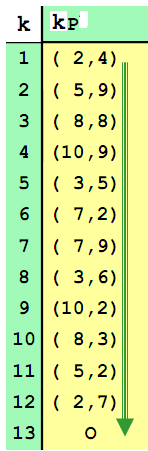
\includegraphics[width=0.85\textwidth]{../../images/python/page_036_img_01.png}

\end{document}
